% Options for packages loaded elsewhere
\PassOptionsToPackage{unicode}{hyperref}
\PassOptionsToPackage{hyphens}{url}
%
\documentclass[
  17pt,
  letterpaper,
  ignorenonframetext,
  aspectratio=169,
]{beamer}
\usepackage{pgfpages}
\setbeamertemplate{caption}[numbered]
\setbeamertemplate{caption label separator}{: }
\setbeamercolor{caption name}{fg=normal text.fg}
\beamertemplatenavigationsymbolsempty
% Prevent slide breaks in the middle of a paragraph
\widowpenalties 1 10000
\raggedbottom
\setbeamertemplate{part page}{
  \centering
  \begin{beamercolorbox}[sep=16pt,center]{part title}
    \usebeamerfont{part title}\insertpart\par
  \end{beamercolorbox}
}
\setbeamertemplate{section page}{
  \centering
  \begin{beamercolorbox}[sep=12pt,center]{part title}
    \usebeamerfont{section title}\insertsection\par
  \end{beamercolorbox}
}
\setbeamertemplate{subsection page}{
  \centering
  \begin{beamercolorbox}[sep=8pt,center]{part title}
    \usebeamerfont{subsection title}\insertsubsection\par
  \end{beamercolorbox}
}
\AtBeginPart{
  \frame{\partpage}
}
\AtBeginSection{
  \ifbibliography
  \else
    \frame{\sectionpage}
  \fi
}
\AtBeginSubsection{
  \frame{\subsectionpage}
}

\usepackage{amsmath,amssymb}
\usepackage{lmodern}
\usepackage{iftex}
\ifPDFTeX
  \usepackage[T1]{fontenc}
  \usepackage[utf8]{inputenc}
  \usepackage{textcomp} % provide euro and other symbols
\else % if luatex or xetex
  \usepackage{unicode-math}
  \defaultfontfeatures{Scale=MatchLowercase}
  \defaultfontfeatures[\rmfamily]{Ligatures=TeX,Scale=1}
  \setmainfont[BoldFont = SF Pro Text Semibold, Scale =
MatchLowercase]{SF Pro Text Light}
\fi
\usecolortheme{wolverine}
\usefonttheme{serif} % use mainfont rather than sansfont for slide text
\useinnertheme{default}
\useoutertheme{miniframes}
% Use upquote if available, for straight quotes in verbatim environments
\IfFileExists{upquote.sty}{\usepackage{upquote}}{}
\IfFileExists{microtype.sty}{% use microtype if available
  \usepackage[]{microtype}
  \UseMicrotypeSet[protrusion]{basicmath} % disable protrusion for tt fonts
}{}
\makeatletter
\@ifundefined{KOMAClassName}{% if non-KOMA class
  \IfFileExists{parskip.sty}{%
    \usepackage{parskip}
  }{% else
    \setlength{\parindent}{0pt}
    \setlength{\parskip}{6pt plus 2pt minus 1pt}}
}{% if KOMA class
  \KOMAoptions{parskip=half}}
\makeatother
\usepackage{xcolor}
\newif\ifbibliography
\setlength{\emergencystretch}{3em} % prevent overfull lines
\setcounter{secnumdepth}{-\maxdimen} % remove section numbering


\providecommand{\tightlist}{%
  \setlength{\itemsep}{0pt}\setlength{\parskip}{0pt}}\usepackage{longtable,booktabs,array}
\usepackage{calc} % for calculating minipage widths
\usepackage{caption}
% Make caption package work with longtable
\makeatletter
\def\fnum@table{\tablename~\thetable}
\makeatother
\usepackage{graphicx}
\makeatletter
\def\maxwidth{\ifdim\Gin@nat@width>\linewidth\linewidth\else\Gin@nat@width\fi}
\def\maxheight{\ifdim\Gin@nat@height>\textheight\textheight\else\Gin@nat@height\fi}
\makeatother
% Scale images if necessary, so that they will not overflow the page
% margins by default, and it is still possible to overwrite the defaults
% using explicit options in \includegraphics[width, height, ...]{}
\setkeys{Gin}{width=\maxwidth,height=\maxheight,keepaspectratio}
% Set default figure placement to htbp
\makeatletter
\def\fps@figure{htbp}
\makeatother

\captionsetup[figure]{labelformat=empty}
\usepackage{pgfpages}
\setbeamertemplate{itemize item}[circle]
\setbeamertemplate{footline}[frame number]{}
\mode<handout>{\pgfpagesuselayout{6 on 1}[letterpaper, border shrink=8mm]}
\AtBeginSection{%
   \begin{frame}
       \tableofcontents[currentsection]
   \end{frame}
}
\makeatletter
\makeatother
\makeatletter
\makeatother
\makeatletter
\@ifpackageloaded{caption}{}{\usepackage{caption}}
\AtBeginDocument{%
\ifdefined\contentsname
  \renewcommand*\contentsname{Table of contents}
\else
  \newcommand\contentsname{Table of contents}
\fi
\ifdefined\listfigurename
  \renewcommand*\listfigurename{List of Figures}
\else
  \newcommand\listfigurename{List of Figures}
\fi
\ifdefined\listtablename
  \renewcommand*\listtablename{List of Tables}
\else
  \newcommand\listtablename{List of Tables}
\fi
\ifdefined\figurename
  \renewcommand*\figurename{Figure}
\else
  \newcommand\figurename{Figure}
\fi
\ifdefined\tablename
  \renewcommand*\tablename{Table}
\else
  \newcommand\tablename{Table}
\fi
}
\@ifpackageloaded{float}{}{\usepackage{float}}
\floatstyle{ruled}
\@ifundefined{c@chapter}{\newfloat{codelisting}{h}{lop}}{\newfloat{codelisting}{h}{lop}[chapter]}
\floatname{codelisting}{Listing}
\newcommand*\listoflistings{\listof{codelisting}{List of Listings}}
\makeatother
\makeatletter
\@ifpackageloaded{caption}{}{\usepackage{caption}}
\@ifpackageloaded{subcaption}{}{\usepackage{subcaption}}
\makeatother
\makeatletter
\@ifpackageloaded{tcolorbox}{}{\usepackage[many]{tcolorbox}}
\makeatother
\makeatletter
\@ifundefined{shadecolor}{\definecolor{shadecolor}{rgb}{.97, .97, .97}}
\makeatother
\makeatletter
\makeatother
\ifLuaTeX
  \usepackage{selnolig}  % disable illegal ligatures
\fi
\IfFileExists{bookmark.sty}{\usepackage{bookmark}}{\usepackage{hyperref}}
\IfFileExists{xurl.sty}{\usepackage{xurl}}{} % add URL line breaks if available
\urlstyle{same} % disable monospaced font for URLs
\hypersetup{
  pdftitle={Knowledge and Reality, Lecture 07},
  pdfauthor={Brian Weatherson},
  hidelinks,
  pdfcreator={LaTeX via pandoc}}

\title{Knowledge and Reality, Lecture 07}
\author{Brian Weatherson}
\date{2022-09-21}

\begin{document}
\frame{\titlepage}
\ifdefined\Shaded\renewenvironment{Shaded}{\begin{tcolorbox}[interior hidden, sharp corners, boxrule=0pt, enhanced, borderline west={3pt}{0pt}{shadecolor}, breakable, frame hidden]}{\end{tcolorbox}}\fi

\hypertarget{srinivasan}{%
\section{Srinivasan}\label{srinivasan}}

\begin{frame}{Short Version}
\protect\hypertarget{short-version}{}
\begin{itemize}[<+->]
\tightlist
\item
  In cases involving accurate beliefs under oppressive circumstances,
  reliability is enough for rationality.
\item
  So internalism is false as applied to these rather important actual
  cases.
\end{itemize}
\end{frame}

\begin{frame}{Three Cases}
\protect\hypertarget{three-cases}{}
\begin{enumerate}[<+->]
\tightlist
\item
  Instinctive correct belief.
\item
  Instinctive correct belief which persists despite counter-evidence.
\item
  False belief that matches lots of testimony.
\end{enumerate}
\end{frame}

\begin{frame}{Three Rival Theories}
\protect\hypertarget{three-rival-theories}{}
\begin{itemize}[<+->]
\tightlist
\item
  Internalism.
\item
  This is incompatible with all of the cases.
\end{itemize}
\end{frame}

\begin{frame}{Three Rival Theories}
\protect\hypertarget{three-rival-theories-1}{}
\begin{itemize}[<+->]
\tightlist
\item
  Process reliabilism, with the defeater condition.
\item
  This is incompatible with the second case.
\end{itemize}
\end{frame}

\begin{frame}{Three Rival Theories}
\protect\hypertarget{three-rival-theories-2}{}
\begin{itemize}[<+->]
\tightlist
\item
  I don't know of anyone who has this view, but the third case seems
  designed to oppose a view that someone probably should have.
\item
  Call it the generous view of rationality.
\end{itemize}
\end{frame}

\begin{frame}{Three Rival Theories}
\protect\hypertarget{three-rival-theories-3}{}
Here's how the `generous' view (my term) works. A belief is rational iff
it is:

\begin{enumerate}[<+->]
\tightlist
\item
  Formed by a reliable process; or
\item
  Properly based in the evidence.
\end{enumerate}
\end{frame}

\begin{frame}{Three Rival Theories}
\protect\hypertarget{three-rival-theories-4}{}
No one has this view, but it seems interesting because it gets a lot of
cases right, especially evil demon cases.

\begin{itemize}[<+->]
\tightlist
\item
  But it gets the third of Srinivasan's cases wrong.
\end{itemize}
\end{frame}

\begin{frame}{Case Judgments}
\protect\hypertarget{case-judgments}{}
What do \textbf{you} think about the three cases?
\end{frame}

\begin{frame}{Argument Structure}
\protect\hypertarget{argument-structure}{}
What role do the cases play in Srinivasan's theory?

\begin{enumerate}[<+->]
\tightlist
\item
  Trigger snap reactions that theory is judged against?
\item
  Make us reflect on what we want a theory of good belief for?
\end{enumerate}
\end{frame}

\begin{frame}{Argument Structure}
\protect\hypertarget{argument-structure-1}{}
\begin{itemize}[<+->]
\tightlist
\item
  My (idiosyncratic) view is that 1 isn't a very good reason to think
  about cases like these.
\item
  But 2 could be a good reason.
\end{itemize}
\end{frame}

\begin{frame}{Cases and Principles}
\protect\hypertarget{cases-and-principles}{}
What general lessons about belief can we draw from reflection on these
kinds of cases?
\end{frame}

\begin{frame}{Cues}
\protect\hypertarget{cues}{}
On the next slide is one kind of argument I think can be drawn from
these cases (not sure if it's a fair reading of the paper though).
\end{frame}

\begin{frame}{Cues}
\protect\hypertarget{cues-1}{}
\begin{enumerate}[<+->]
\tightlist
\item
  Rational, justified belief is a matter of doing well in believing.
\item
  Doing well in believing, for creatures like us, involves picking up on
  subtle cues.
\item
  This is often something that is not available to consciousness, or
  available to reasoning.
\item
  So rationality isn't just about reasoning from conscious states.
\end{enumerate}
\end{frame}

\begin{frame}{Racists and Clairvoyants}
\protect\hypertarget{racists-and-clairvoyants}{}
To end, let's look at Srinivasan's argument that her examples generalise
to promote a simple, or what she calls \textbf{radical} externalism.

\begin{itemize}[<+->]
\tightlist
\item
  I found this part of the argument rather odd.
\end{itemize}
\end{frame}

\begin{frame}{Argument by Analogy}
\protect\hypertarget{argument-by-analogy}{}
\begin{enumerate}[<+->]
\tightlist
\item
  Nour is justified in believing her host is racist.
\item
  Nour's case is just like Bonjour's case of Norman.
\item
  So Norman is justified in his clairvoyant beliefs.
\end{enumerate}
\end{frame}

\begin{frame}{Argument by Analogy}
\protect\hypertarget{argument-by-analogy-1}{}
\begin{itemize}[<+->]
\tightlist
\item
  Why should we believe premise 2 here?
\item
  I know why an \textbf{internalist} should believe it, by stipulation
  the cases are pretty similar from the inside, but why should an
  \textbf{externalist} believe it?
\end{itemize}
\end{frame}

\begin{frame}{Disanalogies}
\protect\hypertarget{disanalogies}{}
\begin{itemize}[<+->]
\tightlist
\item
  The Nour example is pretty realistic, the Norman case is totally not.
\item
  There is an explanation for why Nour could have this ability; there is
  no explanation for Norman.
\item
  Nour's ability is widespread; Norman's is idiosyncratic.
\end{itemize}
\end{frame}

\begin{frame}{Group Externalism}
\protect\hypertarget{group-externalism}{}
So here's a view that is untouched by Srinivasan's example, but agrees
with Bonjour about Norman.

\begin{itemize}[<+->]
\tightlist
\item
  A belief is justified iff it is produced by a process that is
  reliable, and widely shared among similar people.
\end{itemize}
\end{frame}

\begin{frame}{Group Externalism}
\protect\hypertarget{group-externalism-1}{}
This could obviously do with some more care about the details - I
literally just made it up - but it feels more natural given the Marxist
motivations to think about groups than individual reliability.
\end{frame}

\hypertarget{analysis}{%
\section{Analysis}\label{analysis}}

\begin{frame}{What is Knowledge?}
\protect\hypertarget{what-is-knowledge}{}
Question: What conditions are both \textbf{necessary} and
\textbf{sufficient} for knowledge.
\end{frame}

\begin{frame}{Necessary Conditions}
\protect\hypertarget{necessary-conditions}{}
\begin{itemize}[<+->]
\tightlist
\item
  These conditions are needed for knowledge.
\item
  In any case of knowledge, these conditions obtain.
\end{itemize}
\end{frame}

\begin{frame}{Sufficient Conditions}
\protect\hypertarget{sufficient-conditions}{}
\begin{itemize}[<+->]
\tightlist
\item
  These conditions suffice for knowledge.
\item
  If you meet all of them, you know.
\end{itemize}
\end{frame}

\begin{frame}{Dream}
\protect\hypertarget{dream}{}
Some conditions such that:

\begin{itemize}[<+->]
\tightlist
\item
  Each of them on their own is necessary.
\item
  Between them, they are sufficient.
\end{itemize}
\end{frame}

\begin{frame}{Example}
\protect\hypertarget{example}{}
The following are all necessary conditions on being a square, and
between them they are sufficient.

\begin{itemize}[<+->]
\tightlist
\item
  Quadrilateral.
\item
  Equal sides.
\item
  Equal angles.
\end{itemize}
\end{frame}

\begin{frame}{Analysis}
\protect\hypertarget{analysis-1}{}
In this way we've analysed the concept of being a square, just like a
chemist might analyse water into Hydrogen and Oxygen.

\begin{itemize}[<+->]
\tightlist
\item
  Can this kind of analysis, modeled on the great successes of early C20
  chemistry, work for more concepts than geometric ones?
\item
  Can it work for knowledge?
\end{itemize}
\end{frame}

\begin{frame}{Spoiler Alert}
\protect\hypertarget{spoiler-alert}{}
No
\end{frame}

\hypertarget{the-jtb-theory}{%
\section{The JTB Theory}\label{the-jtb-theory}}

\begin{frame}{A Theory Schema}
\protect\hypertarget{a-theory-schema}{}
S knows that \(p\) iff the following conditions are met:

\begin{itemize}[<+->]
\tightlist
\item
  S believes that \(p\).
\item
  \(p\) is true.
\item
  S's belief is rational/justified.
\end{itemize}
\end{frame}

\begin{frame}{JTB}
\protect\hypertarget{jtb}{}
In short, S has a Justified True Belief that \(p\).

\begin{itemize}[<+->]
\tightlist
\item
  This became known as the JTB theory.
\end{itemize}
\end{frame}

\begin{frame}{JTB}
\protect\hypertarget{jtb-1}{}
\begin{itemize}[<+->]
\tightlist
\item
  Fun fact: although it gets talked about a lot, it's not clear anyone
  ever held exactly that theory.
\item
  The terminology comes from Ed Gettier's 1963 paper ``Is Justified True
  Belief Knowledge?''.
\item
  But Gettier is using ``justified'' as a shorthand for a few different
  things that could go in place of third condition.
\end{itemize}
\end{frame}

\begin{frame}{Gettier}
\protect\hypertarget{gettier}{}
The short paper you've seen is one of the most cited in contemporary
philosophy.

\begin{itemize}[<+->]
\tightlist
\item
  It launched the ``Gettier problem'', which was the problem of either
  adding to, or replacing, one of those three conditions to get the
  analysis right.
\item
  Nowadays the general view is that the problem can't be solved, but it
  was a big deal.
\end{itemize}
\end{frame}

\begin{frame}{The Gettier Problem}
\protect\hypertarget{the-gettier-problem}{}
You'll often see people say that this was what epistemologists talked
about in the late 20C.

\begin{itemize}[<+->]
\tightlist
\item
  Pasnau very often alludes to this, for example.
\item
  I don't think the data backs this up.
\end{itemize}
\end{frame}

\begin{frame}{Some Data}
\protect\hypertarget{some-data}{}
\begin{figure}

{\centering 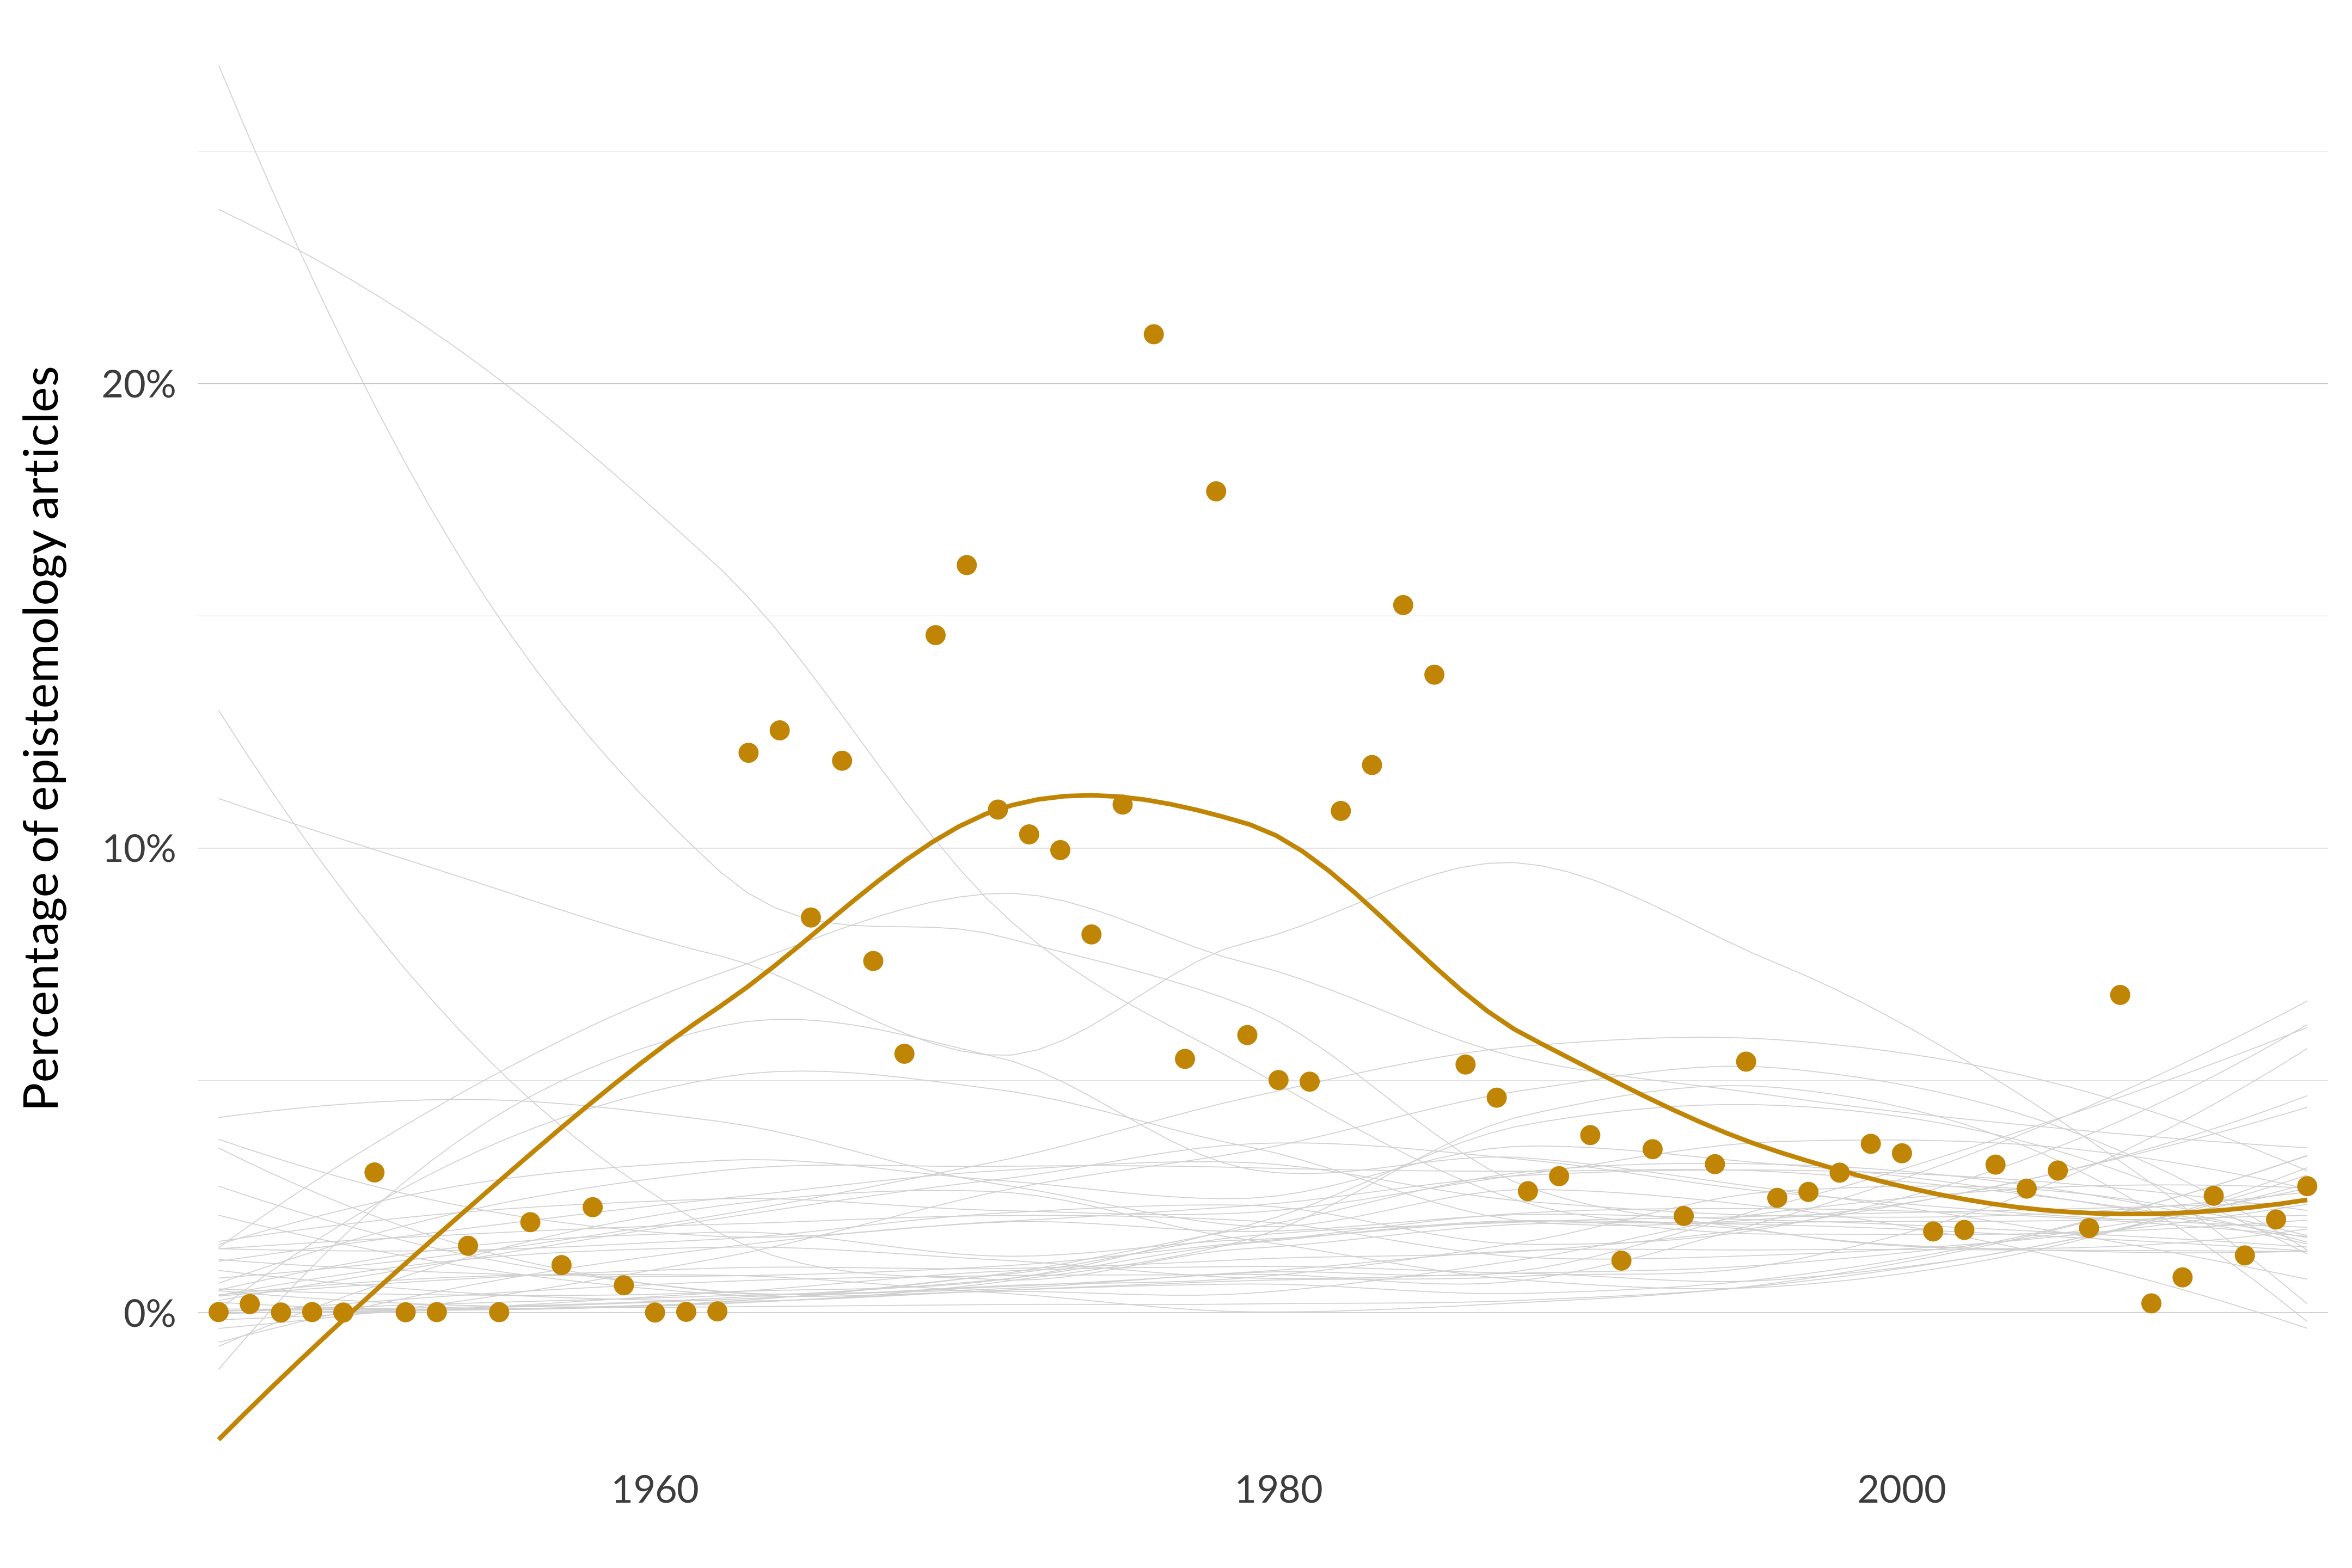
\includegraphics[width=\textwidth,height=0.6\textheight]{../images/gettier-percent.png}

}

\caption{Percentage of epistemology articles each year that were on
Gettier problem}

\end{figure}
\end{frame}

\hypertarget{two-cases}{%
\section{Two Cases}\label{two-cases}}

\begin{frame}{Two Cases}
\protect\hypertarget{two-cases-1}{}
I'm going to go over one case from Gettier, and one from the 9th century
philosopher Dharmattara.
\end{frame}

\begin{frame}{Gettier Example}
\protect\hypertarget{gettier-example}{}
\begin{itemize}[<+->]
\tightlist
\item
  Smith believes, on good evidence, that Brown is in Barcelona.
\item
  Brown is not in Barcelona.
\item
  Smith has just learned in logic class that from A, we can always infer
  A or B.
\item
  So Smith infers Brown is in Barcelona or he's in Bordeaux.
\item
  By complete coincidence, Brown is in Bordeaux.
\end{itemize}
\end{frame}

\begin{frame}{Question}
\protect\hypertarget{question}{}
Does Smith know that Brown is in Barcelona or Bordeaux.
\end{frame}

\begin{frame}{Generalisation}
\protect\hypertarget{generalisation}{}
\begin{itemize}[<+->]
\tightlist
\item
  Take any justified false belief that \(p\).
\item
  Imagine the believer infers both \(p \vee q\) and \(p \vee \neg q\).
\item
  One of these is true!
\item
  Is it a piece of knowledge.
\end{itemize}
\end{frame}

\begin{frame}{Dharmattara Example}
\protect\hypertarget{dharmattara-example}{}
\begin{itemize}[<+->]
\tightlist
\item
  A traveller sees a black cloud the other side of a hill.
\item
  It looks like smoke, and he infers that it is smoke.
\item
  By a well known rule, he infers there is a fire over the hill.
\item
  There is a fire, but that's not smoke.
\item
  It's the swarm of flies that have gathered over the fire.
\end{itemize}
\end{frame}

\begin{frame}{Question}
\protect\hypertarget{question-1}{}
Does the traveller know that there is a fire over the hill?
\end{frame}

\hypertarget{two-lessons}{%
\section{Two Lessons}\label{two-lessons}}

\begin{frame}{Lesson from Dharmottara}
\protect\hypertarget{lesson-from-dharmottara}{}
Causation isn't enough.
\end{frame}

\begin{frame}{A Proposed Theory}
\protect\hypertarget{a-proposed-theory}{}
S knows that \(p\) just in case

\begin{itemize}[<+->]
\tightlist
\item
  S believes that \(p\).
\item
  \(p\) is true.
\item
  S's belief is rational/justified.
\item
  S's belief is caused by \(p\).
\end{itemize}
\end{frame}

\begin{frame}{Problem}
\protect\hypertarget{problem}{}
The traveler's belief satisfies all these conditions!
\end{frame}

\begin{frame}{Lesson from Gettier}
\protect\hypertarget{lesson-from-gettier}{}
Linda Zagzebski pointed out that the original example worked against a
very broad range of theories.
\end{frame}

\begin{frame}{Zagzebski}
\protect\hypertarget{zagzebski}{}
Consider a theory that says S knows that \(p\) just in case

\begin{itemize}[<+->]
\tightlist
\item
  S believes that \(p\).
\item
  \(p\) is true.
\item
  S's belief has feature F, where F (a) is preserved by logical
  inference, and (b) does not imply truth.
\end{itemize}
\end{frame}

\begin{frame}{Zagzebski}
\protect\hypertarget{zagzebski-1}{}
For almost F, there's a Brown in Barcelona example.

\begin{itemize}[<+->]
\tightlist
\item
  Make the belief that Brown is in Barcelona have feature F.
\item
  Make it be true (but completely unknown) that Brown is in Bordeaux.
\item
  Then Brown is in Barcelona or Bordeaux will be F.
\item
  But it won't be knowledge.
\end{itemize}
\end{frame}

\begin{frame}{Two Ways Out}
\protect\hypertarget{two-ways-out}{}
\begin{enumerate}[<+->]
\tightlist
\item
  Make F not be closed under logical inference.
\item
  Make F imply truth.
\end{enumerate}

\begin{itemize}[<+->]
\tightlist
\item
  These are not incompatible; you could do both!
\end{itemize}
\end{frame}

\begin{frame}{For Next Time}
\protect\hypertarget{for-next-time}{}
Look at some theories that take one or both of these options.
\end{frame}



\end{document}
